\chapter{Introduction}\label{chap:introduction}

Les documents scientifiques qui reflètent l'état des connaissances des domaines des sciences sont stockés dans des bibliothèques numériques scientifiques.
% accéder / rechercher ??
Pour pouvoir rechercher ces documents, il faut qu'ils soient au préalable indexés par leur contenu, que ce soit par l'entièreté du texte ou par des mots-clés.
Les mots-clés représentent les concepts les plus importants d'un document et servent de condensateur textuel, c'est-à-dire qu'ils sont \say{une expression du texte à la fois réduite du point de vue de la forme et synthétique du point de vue de son \say{sens}}~\cite{amar_les_1997}.
Ils sont le plus souvent utilisés directement pour indexer des documents mais ils servent aussi à la détection d'opinion~\cite{berend_opinion_2011}, à la catégorisation de texte~\cite{hulth_study_2006} ou encore à l'élaboration automatique de résumés~\cite{zhang_world_2004}.

\begin{figure}[!htbp]
    \begin{subfigure}{.5\textwidth}
        \centering
        \label{fig:pubmed_submission_per_year}
        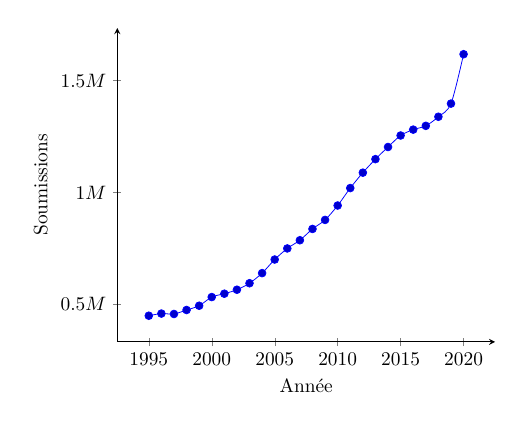
\begin{tikzpicture}[scale=0.7, transform shape]
        \begin{axis}[
        scaled y ticks=manual:{}{\pgfmathparse{#1/1000000}},
        axis x line=bottom, axis y line=left,
        enlargelimits=true,
        yticklabel=${\pgfmathprintnumber{\tick}M}$,
        xlabel=\text{Année},ylabel=\text{Soumissions},
        x tick label style={
            /pgf/number format/.cd, use comma, 1000 sep={},
        }]
        \addplot+[smooth] coordinates {
            (1995, 449050)(1996, 458678)(1997, 456812)(1998, 474666)(1999, 493712)(2000, 532503)(2001, 547504)(2002, 565256)(2003, 594340)(2004, 639530)(2005, 700229)(2006, 749769)(2007, 786530)(2008, 836935)(2009, 877310)(2010, 941684)(2011, 1019685)(2012, 1088548)(2013, 1148929)(2014, 1203202)(2015, 1254639)(2016, 1280910)(2017, 1297742)(2018, 1338381)(2019, 1397240)(2020, 1617944)
            };    
        \end{axis}
        \end{tikzpicture}
        \caption{PubMed}
    \end{subfigure}%
    %
    \begin{subfigure}{.5\textwidth}
        \centering
        \label{fig:arxiv_submission_per_year}
        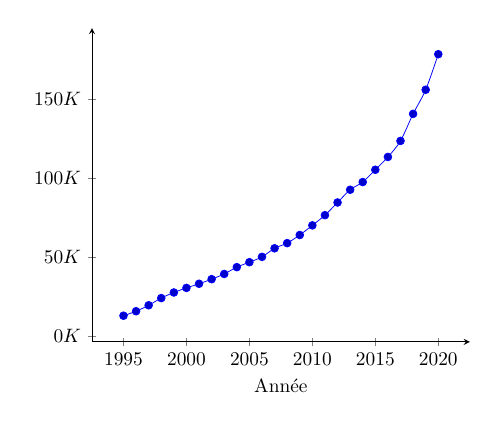
\begin{tikzpicture}[scale=0.7, transform shape]
        \begin{axis}[
            scaled y ticks=manual:{}{\pgfmathparse{#1/1000}},
            axis x line=bottom, axis y line=left,
            enlargelimits=true,
            yticklabel=${\pgfmathprintnumber{\tick}K}$,
            xlabel={Année},%ylabel=\text{Soumissions},
            x tick label style={
                /pgf/number format/.cd, use comma, 1000 sep={},
            }]
        \addplot+[smooth] coordinates {
            %(1991, 306)(1992, 3263)(1993, 6743)(1994, 10097)
            (1995, 13014)(1996, 15866)(1997, 19624)(1998, 24172)(1999, 27704)(2000, 30601)(2001, 33214)(2002, 36121)(2003, 39414)(2004, 43727)(2005, 46855)(2006, 50227)(2007, 55638)(2008, 58915)(2009, 64047)(2010, 70131)(2011, 76578)(2012, 84603)(2013, 92641)(2014, 97517)(2015, 105280)(2016, 113380)(2017, 123523)(2018, 140616)(2019, 155866)(2020, 178329)
            };    
        \end{axis}
        \end{tikzpicture}
        \centering
        \caption{ArXiv}
    \end{subfigure}%
    
    \iffalse
    \begin{subfigure}{.5\textwidth}
        \centering
        \label{fig:hal_submission_per_year}
        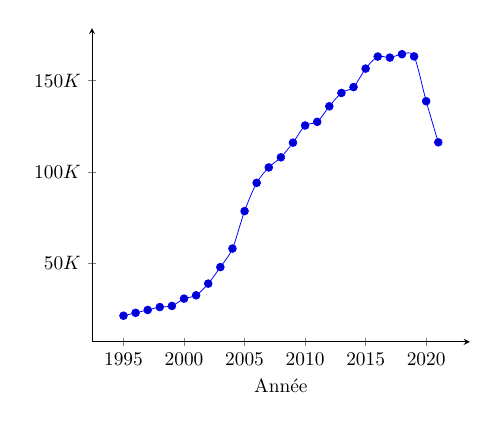
\begin{tikzpicture}[scale=0.7, transform shape]
        \begin{axis}[
            scaled y ticks=manual:{}{\pgfmathparse{#1/1000}}, 
            axis x line=bottom, axis y line=left,
            enlargelimits=true,
            yticklabel=${\pgfmathprintnumber{\tick}K}$,
            xlabel={Année},%ylabel=\text{Soumissions},
            x tick label style={
                /pgf/number format/.cd, use comma, 1000 sep={},
            }]
        \addplot+[smooth] coordinates {
            (2021, 116139)(2020, 138691)(2019, 163279)(2018, 164475)(2017, 162607)(2016, 163185)(2015, 156587)(2014, 146438)(2013, 143213)(2012, 135893)(2011, 127362)(2010, 125351)(2009, 115950)(2008, 107903)(2007, 102352)(2006, 93887)(2005, 78390)(2004, 57840)(2003, 47662)(2002, 38605)(2001, 32185)(2000, 30366)(1999, 26367)(1998, 25741)(1997, 24139)(1996, 22571)(1995, 20987)
            };    
        \end{axis}
        \end{tikzpicture}
        \centering
        \caption{HAL}
    \end{subfigure}
    \fi
    
    \caption{Nombre de nouveaux documents par an dans deux bibliothèques numériques scientifiques.}
    \label{fig:submission_per_year}
\end{figure}

Le nombre de documents que contiennent les bibliothèques numériques scientifiques ne cesse d'augmenter.
La figure~\ref{fig:submission_per_year} illustre la croissance exponentielle du nombre de documents déposés chaque année dans ces bibliothèques.
\`A titre d'exemple, plus de $180\,000$ documents ont été déposés dans la bibliothèque ArXiV en 2020 contre seulement $100\,000$ en 2015.\footnote{Les données de ArXiV et de PubMed proviennent respectivement de \url{https://arxiv.org/stats/get_monthly_submissions} et \url{https://pubmed.ncbi.nlm.nih.gov/?term=all[sb]}.}
%
Ainsi, le nombre d'articles retournés pour une requête précise augmente avec ce nombre croissant de documents et rend plus laborieuse la recherche documentaire.
Des moteurs de recherche dédiés facilitent néanmoins cette recherche de documents scientifiques, comme Google Scholar qui est le plus populaire ou encore Microsoft Academics et SemanticScholar. Ces derniers permettent de filtrer une partie des documents grâce à l'identification automatique de \say{sujets} dans les documents.

%L'indexation manuelle, réalisée par des documentalistes, pose des problèmes  en termes de coûts, de disponibilité d'experts et de masse de données à traiter.
L'annotation manuelle, réalisée par des documentalistes, atteint ses limites lorsque la masse de documents à traiter est trop importante, d'une part pour être absorbée par les experts disponibles, d'autre part en termes de coût.
C'est pourquoi, l'indexation de grandes quantités de documents par mots-clés est aujourd'hui semi-~\cite{mork_nlm_2013} ou totalement automatique~\cite{cuxac_archives_2017}.
%C'est pourquoi, l'indexation de grandes quantités de documents par mots-clés nécessite d'être automatisée.
%Aujourd'hui cette indexation est semi-~\cite{mork_nlm_2013} ou totalement automatique~\cite{cuxac_archives_2017}.
La production automatique de mots-clés pour un document est une thématique à part entière qui mobilise plusieurs communautés scientifiques dont celle du traitement automatique des langues qui s'y intéresse depuis les années soixante-dix.
Les travaux pionniers de Karen Spärck Jones permettent d'identifier les mots importants d'un document grâce à l'introduction de la mesure de \tfidf{}~\cite{jones_statistical_1972}.
% Qu'est-ce qu'il faut faire
La production de mots-clés pour un document consiste d'abord à identifier les concepts importants, puis à ne retenir qu'un certain nombre de ces concepts selon divers critères et enfin à choisir une dénomination de ces concepts parmi toutes les formes linguistiques possibles.
% Pourquoi c'est pas facile ?
Ces étapes nécessitent une expertise tant sur le domaine du document que dans la pratique d'indexation documentaire. En effet l'identification des concepts repose sur une compréhension du document et le choix de leurs dénominations nécessite de respecter certaines caractéristiques linguistiques.
De plus, l'ensemble des mots-clés d'un document doit répondre à des contraintes globales: il doit être complet, c-à-d. qu'il doit couvrir le maximum de concepts importants, et être minimal, c-à-d. que leurs sens doivent se recouvrir le moins possible.
%
Les premières méthodes de production automatique de mots-clés sont extractives, ce qui signifie que les mots-clés sont identifiés à l'intérieur du document. Elles fonctionnent en chaîne de traitement et reposent sur des représentations statistiques ou des graphes pour identifier les mots les plus importants grâce à leur fréquence, leur position ou leur centralité dans le document.

% La présentation des méthodes neuronales est coincée là dedans......
% Difficile à comparer
% Les meth neuronales exacerbent cette difficulté
% Elles ont besoin de grand jeu de données
% Il n'y en a qu'un seul
% En plus l'évaluation est intrinsèque
Les méthodes présentées par la communauté scientifique sont nombreuses mais elles sont difficilement comparables car la plupart sont évaluées sur des données différentes, pré-traitées différemment et selon des protocoles évaluatifs différents.
Ce manque de comparabilité ne permet pas d'orienter efficacement la recherche dans le domaine de la production automatique de mots-clés.
%
De plus, ce phénomène de faible comparabilité est exacerbé par le développement de méthodes neuronales de bout-en-bout. Celles-ci ont la capacité de produire une catégorie de mots-clés qui n'avait jusqu'alors reçu que peu d'attention: les mots-clés absents. Ces méthodes, contrairement aux méthodes extractives en chaîne de traitement, peuvent s'abstraire du document et ne sont plus limités aux seules unités textuelles apparaissant dans le document traité.
%
Ces méthodes de bout-en-bout exploitent l'architecture neuronale encodeur-décodeur qui requiert de grandes quantités de données annotées pour être entraînées.
Malheureusement, il n'existe qu'un seul grand jeu de données permettant cet entraînement ce qui limite l'analyse et la comparaison des méthodes de bout-en-bout.
%
En plus de cette faible comparabilité, la méthode d'évaluation usuelle compare les mots-clés prédits à une référence par correspondance exacte, ce qui résulte en une évaluation pessimiste des performances des méthodes de production automatique de mots-clés.
%En plus de la faible comparabilité, la méthode d'évaluation usuelle calcule un score en comparant de manière exacte les mots-clés prédits à une référence. Cette comparaison exacte qui ne peut prendre en compte des variantes donne des scores pessimiste qui sous-évalue les méthodes.
% pourquoi dire que les références sont incomplètes ? incomplète par rapport à quoi ?
Cette méthode d'évaluation, intrinsèque, ne considère pas l'utilité des mots-clés dans des tâches applicatives, comme la recherche d'information par exemple, alors que leur principal intérêt réside justement dans le fait d'être utilisé pour des tâches applicatives.
%réside justement dans leur utilisation pour des tâches applicatives
%Cette méthode d'évaluation, intrinsèque, considère les mots-clés comme une fin en soi, alors que leur principal intérêt réside dans le fait d'être utilisé pour des tâches applicatives, comme la recherche d'information par exemple.
%Cette méthode d'évaluation contribue à faire considérer la production automatique de mots-clés comme une fin en soi alors que le principal intérêt des mots-clés se trouve dans l'indexation de documents.
%En effet, l'utilité des mots-clés dans des tâches applicatives, telle que la recherche d'information, n'est jamais discutée.

% Mots-clés auteurs
%Pour faciliter la tâche d'indexation, certaines conférences ou revues intègrent dans le style de leurs publication un encart où des mots-clés ou des catégories sont renseignés par les auteurs.\\

% Objectifs
Ainsi, les objectifs de nos travaux sont triples.
Le premier est de démontrer la validité des méthodes de bout-en-bout en les confrontant à différents genres de documents.
Jusqu'à présent ces méthodes n'ont été évaluées que sur un seul jeu de données.
Cet objectif implique la construction de nouvelles ressources contenant assez de documents annotés pour permettre l'apprentissage de ces modèles neuronaux profonds.
%
Le second objectif est de comprendre la stagnation en termes de performances des méthodes de production de mots-clés, qu'elles soient statistiques, fondée sur les graphes ou neuronales. Ceci implique de comparer ces méthodes et ainsi de les évaluer de manière unifiée.
%
Le troisième objectif est de quantifier l'efficacité des méthodes de production de mots-clés pour une tâche de recherche d'information, et ainsi plus généralement de mesurer l'utilité des mots-clés produits automatiquement dans une tâche applicative.\\

% Hypothèses
Pour atteindre ces objectifs, nous faisons quatre hypothèses, présentées ci-dessous.
%
Notre première hypothèse concerne les méthodes de bout-en-bout génératives et la qualité des mots-clés de référence.
Elle porte sur la qualité de l'annotation des mots-clés de référence qui devrait influer sur les performances des modèles appris.
La disponibilité d'un seul jeu de données de grande taille ne permet pas de répondre à ce questionnement. Quelques travaux s'intéressent à entraîner ces modèles avec plus de données de manière non supervisée~\cite{ye_semi-supervised_2018} mais à notre connaissance aucun ne s'intéresse à la qualité des mots-clés de référence.
La création d'un autre jeu de données de taille comparable à l'existant mais contenant des mots-clés de meilleure qualité permettrait d'étudier la capacité de généralisation de ces modèles.
Nous faisons l'hypothèse qu'il est possible de construire automatiquement un jeu de données contenant des mots-clés se rapprochant d'annotations professionnelles et ainsi de consolider les résultats des méthodes neuronales.\\
%
Notre deuxième hypothèse concerne la comparaison des performances des méthodes proposées par la communauté scientifique. Les performances de ces méthodes ne peuvent actuellement pas être comparées car elles sont évaluées suivant des cadres expérimentaux différents, et ainsi, ne permettent pas d'avoir une vision d'ensemble des performances de la tâche de production automatique de mots-clés. Nous faisons l'hypothèse qu'il est possible de proposer un cadre expérimental unifié pour reproduire les expériences et ainsi pouvoir évaluer et comparer les méthodes état-de-l'art.\\
%
Notre troisième hypothèse concerne l'évaluation des méthodes de production automatique de mots-clés. Le seul cadre d'évaluation intrinsèque ne permet pas de mesurer efficacement les performances et l'utilité des méthodes proposées. Quelques travaux s'intéressent néanmoins à améliorer l'évaluation intrinsèque en assouplissant la comparaison avec la référence~\cite{zesch_approximate_2009} ou en l'étendant avec des variantes~\cite{kim_semeval-2010_2010,chan_neural_2019}. Nous faisons l'hypothèse qu'il est possible de définir un protocole expérimental dans le cadre de la recherche d'information pour évaluer les méthodes de production automatiques de mots-clés.\\
%
Notre dernière hypothèse concerne les mots-clés absents que les méthodes de bout-en-bout permettent dorénavant de produire.
Cette catégorie de mots-clés permet, dans le cadre de leur indexation, d'enrichir les documents en y ajoutant de nouveaux mots.
Dans le cadre de la recherche de documents, cet enrichissement permet d'augmenter la couverture des documents retournés.
Ainsi, nous faisons l'hypothèse que ces mots-clés, qui n'apparaissent pas dans les documents, ont un plus grand impact sur l'amélioration des performances des systèmes de recherche d'information, que les mots-clés présents dans les documents.

% Plan
Nous présentons tout d'abord dans le chapitre~\ref{chap:concepts} les concepts importants de cette thèse que sont l'indexation et les mots-clés, ainsi qu'un état de l'art des méthodes automatiques d'extraction de mots-clés.
Le chapitre~\ref{chap:kw_production} présente un état de l'art des méthodes de production automatique de mots-clés de bout-en-bout.
Le chapitre~\ref{chap:framework} présente le cadre expérimental de la production automatique de mots-clés. Nous y présentons les jeux de données utilisés, ainsi que le processus d'évaluation des systèmes.
Le chapitre~\ref{chap:kptimes} présente le jeu de données KPTimes que nous avons créé et grâce auquel nous évaluons la généralisation des méthodes de production automatique de mots-clés.
Dans le chapitre~\ref{chap:large-scale-eval} nous présentons une évaluation comparative des méthodes de l'état de l'art sur différents jeux de données.
Puis, nous nous intéressons dans le chapitre~\ref{chap:ri} à l'impact des mots-clés sur l'indexation de documents scientifiques dans le cadre applicatif de la recherche d'information.
Enfin nous présentons nos conclusions et perspectives dans le chapitre~\ref{chap:conclusion}.



% Indexation
%L'indexation de documents est le processus de définition des descripteurs qui vont être utilisés pour rechercher le document.
%L'indexation de documents dont le texte plein n'est pas disponible sous un format lisible par des programmes informatique se fait manuellement grâce à un langage documentaire qui contraint les descripteurs à utiliser.
%Ce travail de définition du langage documentaire est complexe mais permet une indexation cohérente et facilite la recherche en traduisant la requête dans le langage documentaire.
%Aujourd'hui, les moteurs de recherches utilisent les mots du texte comme descripteurs, ce qui permet d'indexer automatiquement les documents.
%Ces techniques nécessitent de disposer du document complet ou de la notice (avec titre et résumé).


% RI
%\begin{quote}
%    La recherche d'information (RI) consiste à trouver de la matière (généralement des documents) de nature non-structurée (généralement du texte) qui répond à un besoin d'information au sein de grandes collections (généralement stockées sur des ordinateurs). Traduction de \citet{manning_introduction_2009}.
%    \small{\emph{Information retrieval (IR) is finding material (usually documents) of an unstructured nature (usually text) that satisfies an information need from within large collections (usually stored on computers).} \citet{manning_introduction_2009}}
%\end{quote}


%    tâche
% Extraire un ensembles de mots-clés décrivant un document spécifique indépendemment de son domaine \cite{hulth_improved_2003}
% Extraire un ensemble d'unités lexicales liées au sujets principaux d'un document \cite{hasan_automatic_2014}
% Fournir les informations clés d'un document. \cite{meng_deep_2017}
% Utiles pour la classification, le clustering, la recommandation, l'indexation, la RI et le résumé.
%    Ensemble
% Les mots-clés sont un ensemble d'unités textuelles qui représentent le document \cite{hasan_conundrum_2010}
%     Individuel
% Un mot-clé est un contenu textuel court et concis qui exprime la sémantique principale d'un texte plus long. \cite{meng_deep_2017}
% Les mots-clés donnent une vision globale du document pour décider s'il est pertinent ou non. \cite{frank_domain-specific_1999}
% Les mots-clés sont des métadonnées qui résument et caractérisent le document. \cite{witten_kea:_1999}
% Les mots-clés donnent une vision globale des sujets du document. \cite{caragea_citation-enhanced_2014}

% Moteur de recherche -> indexe des publi et permet de les rechercher à partir de sources de données
% Liens+cit: Google Scholar, RefSeek, PubMed, Baidu Scholar
% Metadata : Microsoft Academic, AMiner, SemanticScholar

% Sources de données
% archive -> contient des document full texte
% ArXiV, HAL, PubMedCentral, ACM, ACLAnthology, CiteSeerX
% BDD bibliographique -> contient des notices scientifiques
% Web Of Science, Scopus, Medline
